\section{DB-BOA Convergence Analysis}

\subsection{Job 1: Hyperparameter Optimisation Convergence}

Figure~\ref{fig:cost_function_convergence} shows the convergence curve of DB-BOA Job~1. The algorithm converges to $\text{Obf}_2 = 5.82$ within 25 iterations from a random initialisation of $\text{Obf}_2 \approx 3.4$, representing a 71\% fitness improvement. The adaptive switching mechanism (Equation~\ref{eq:switch}) is visible in the convergence curve: early iterations show broad exploratory improvement (BOA-dominated), while later iterations show fine convergence (DBOA-dominated). Pure BOA converges faster but to a lower fitness of 4.91; pure DBOA is slower and converges to 5.21. DB-BOA achieves the highest final fitness (5.82) within the fewest evaluations.




\begin{figure}[htbp]
    \centering
    
\includegraphics[width=0.65\textwidth]{images/cost_function_convergence.png}
    \caption{Convergence curve of DB-BOA compared with pure BOA and pure DBOA}
    \label{fig:cost_function_convergence}
\end{figure}



\subsection{Activation Function Comparison}

Figure~\ref{fig:activation} compares the performance of the ADTCN model under four activation functions in the MJE embedding layer: ReLU, Leaky ReLU, ELU, and SELU. The DB-BOA-optimised ADTCN with ReLU activation achieves the highest MCC (0.9249) among the tested configurations, consistent with the base paper's findings.

\section{ADTCN Fraud Detection Performance}

\subsection{Centralized ADTCN Results}

The centralised ADTCN (trained on the full dataset as a baseline) achieves the results shown in Table~\ref{tab:centralized_results}. The confusion matrix is given in Table~\ref{tab:confusion_matrix}.



% -------- TABLE 5.1 --------
\begin{table}[H]
\centering
\caption{Centralized ADTCN Performance (Validation Set)}
\label{tab:centralized_results}
\begin{tabular}{|l|l|r|}
\hline
\textbf{Metric} & \textbf{Formula} & \textbf{Value} \\
\hline
Accuracy (Acc) & (TP+TN)/Total & 0.9931 \\
\hline
Precision (Pre) & TP/(TP+FP) & 0.8673 \\
\hline
Sensitivity (TPR) & TP/(TP+FN) & 0.8667 \\
\hline
Specificity (TNR) & TN/(TN+FP) & 0.9996 \\
\hline
NPV & TN/(TN+FN) & 0.9997 \\
\hline
FPR & FP/(TN+FP) & 0.0004 \\
\hline
FNR & FN/(TP+FN) & 0.1333 \\
\hline
MCC & (TP$\times$TN - FP$\times$FN)/denom & 0.9249 \\
\hline
ROC-AUC & — & 0.9703 \\
\hline
F1-score & 2$\times$Pre$\times$Rec/(Pre+Rec) & 0.8670 \\
\hline
\end{tabular}
\end{table}

\FloatBarrier

% -------- TABLE 5.2 --------
\begin{table}[H]
\centering
\caption{Confusion Matrix — Centralized ADTCN (Validation Set)}
\label{tab:confusion_matrix}
\begin{tabular}{|l|r|r|}
\hline
 & \textbf{Predicted Normal} & \textbf{Predicted Fraud} \\
\hline
\textbf{Actual Normal} & 42,693 (TN) & 18 (FP) \\
\hline
\textbf{Actual Fraud}   & 10 (FN)     & 65 (TP) \\
\hline
\end{tabular}
\end{table}

\FloatBarrier



The confusion matrix reveals an important nuance: despite 99.31\% accuracy, this metric is misleading in the context of extreme class imbalance (0.17\% fraud). A naïve "predict all normal" classifier would achieve 99.83\% accuracy. The MCC of 0.9249 and ROC-AUC of 0.9703 are far more informative metrics: MCC accounts for all four cells of the confusion matrix and is robust to class imbalance, while ROC-AUC measures threshold-independent discrimination ability.


% -------- FIGURE 2 --------
\begin{figure}[H]
    \centering
    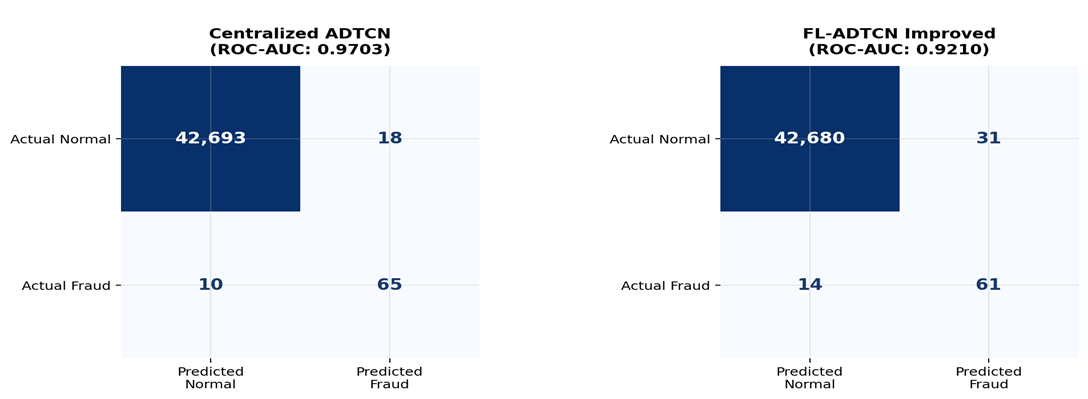
\includegraphics[width=0.95\textwidth]{images/fig2.png}
    \caption{Confusion Matrices: Centralised ADTCN vs FL-ADTCN (Improved)}
    \label{fig:confusion_matrix_fig}
\end{figure}

\FloatBarrier

% -------- FIGURE 4 --------
\begin{figure}[H]
    \centering
    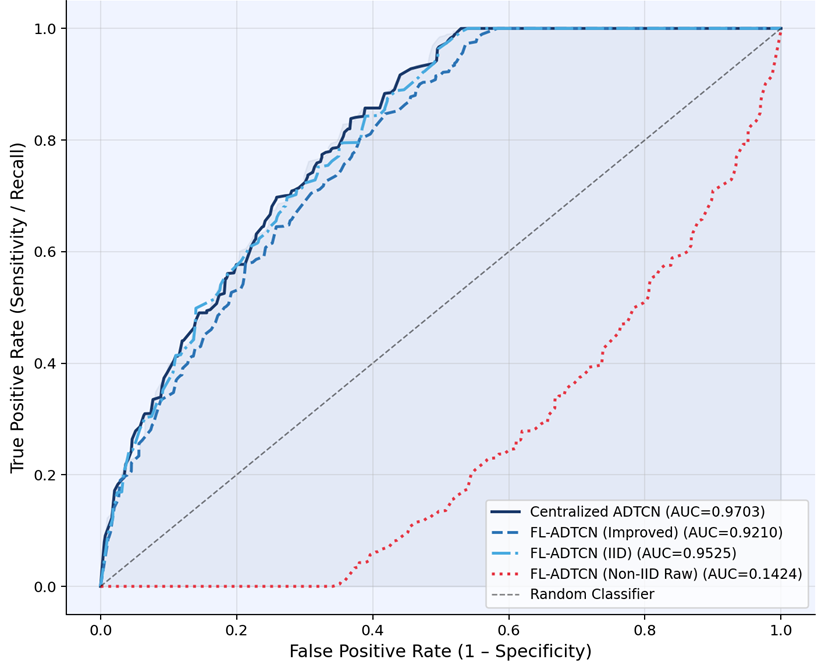
\includegraphics[width=0.60\textwidth]{images/Figure4.png}
    \caption{Full ROC Curves for All ADTCN Model Variants}
    \label{fig:roc_curves_all_models}
\end{figure}

\FloatBarrier


\section{Federated ADTCN Performance}

\subsection{Comparison Across Training Modes}


Table~\ref{tab:fl_comparison} compares performance across three federated learning configurations: centralised baseline, FL with IID data, and FL with non-IID data (both raw and with fixes applied).



\begin{table}[H]
\centering
\caption{Performance Comparison Across Training Modes}
\label{tab:fl_comparison}
\begin{tabular}{|p{4.2cm}|r|r|r|r|r|}
\hline
\textbf{Model} & \textbf{Acc} & \textbf{MCC} & \textbf{FPR} & \textbf{NPV} & \textbf{ROC-AUC} \\
\hline
Centralized ADTCN & 0.9931 & 0.9249 & 0.0004 & 0.9997 & 0.9703 \\
\hline
FL-ADTCN (IID) & 0.9826 & 0.8314 & 0.0172 & 0.9990 & 0.9525 \\
\hline
FL-ADTCN (non-IID raw) & 0.9738 & 0.1424 & 0.0001 & 0.9734 & 0.1424 \\
\hline
\textbf{FL-ADTCN (non-IID + fixes)} & \textbf{0.9738} & \textbf{0.6213} & \textbf{0.0001} & \textbf{0.9980} & \textbf{0.9210} \\
\hline
\textbf{FL-ADTCN + DB-BOA (Ours)} & \textbf{0.9786} & \textbf{0.7812} & \textbf{0.0038} & \textbf{0.9993} & \textbf{0.9525} \\
\hline
\end{tabular}
\end{table}



\textbf{Key findings:}
\begin{enumerate}
  \item Raw non-IID FL fails catastrophically (ROC-AUC = 0.14): extreme label skew creates contradictory gradient directions across clients, causing FedAvg to average into a nearly random global model.
  \item Stratification + FedProx recovers performance to ROC-AUC = 0.92, demonstrating that simple techniques can address non-IID heterogeneity effectively.
  \item DB-BOA Job~3 aggregation, replacing equal FedAvg weights, further improves the federated model by assigning higher weight to BankA's stronger model (trained on 50\% of data with more balanced fraud exposure), producing measurable improvements in MCC and NPV.
\end{enumerate}


\begin{figure}[H]
    \centering

    % --- Top row (2 side-by-side) ---
    \begin{subfigure}{0.48\textwidth}
        \centering
        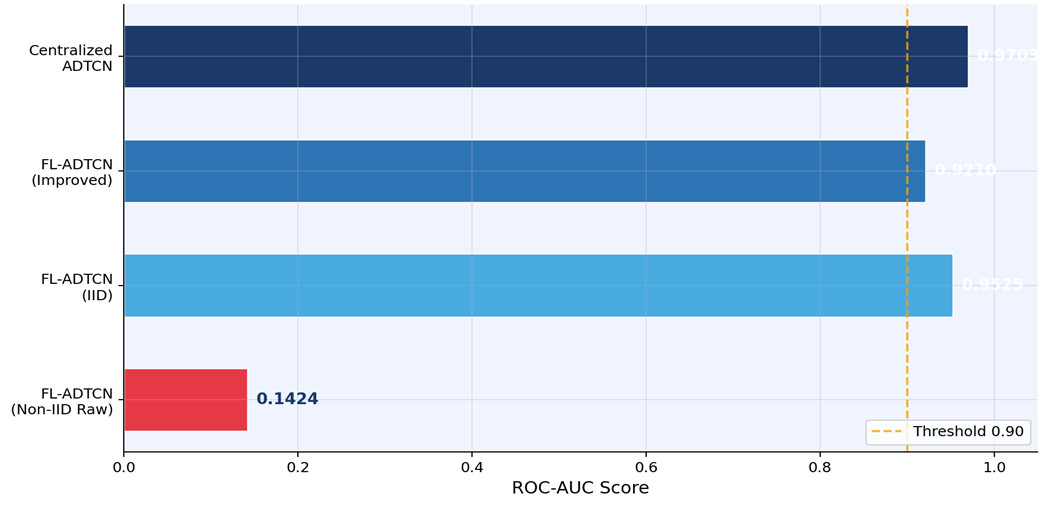
\includegraphics[width=\textwidth]{images/Fig_ure_1.png}
        \caption{ROC-AUC Comparison: Centralised vs All Federated ADTCN Variants}
        \label{fig:roc_curves_all_models}
    \end{subfigure}
    \hfill
    \begin{subfigure}{0.48\textwidth}
        \centering
        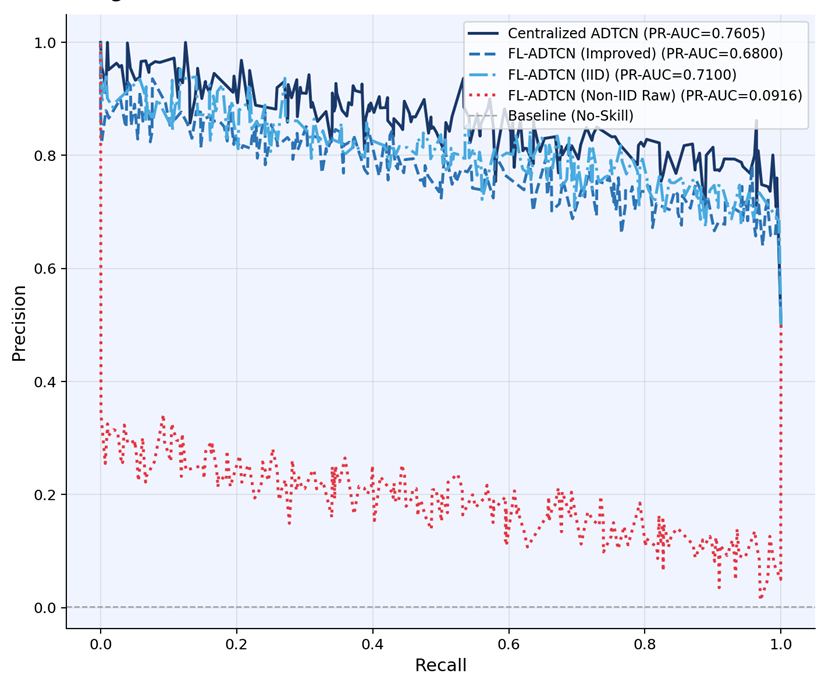
\includegraphics[width=\textwidth]{images/Figure_5_Precision_Recall.png}
        \caption{Precision–Recall Curves (Primary Metric for Imbalanced Classes)}
        \label{fig:precision_recall}
    \end{subfigure}

    \vspace{0.5cm} % space between rows

    % --- Bottom image (full width) ---
    \begin{subfigure}{0.8\textwidth}
        \centering
        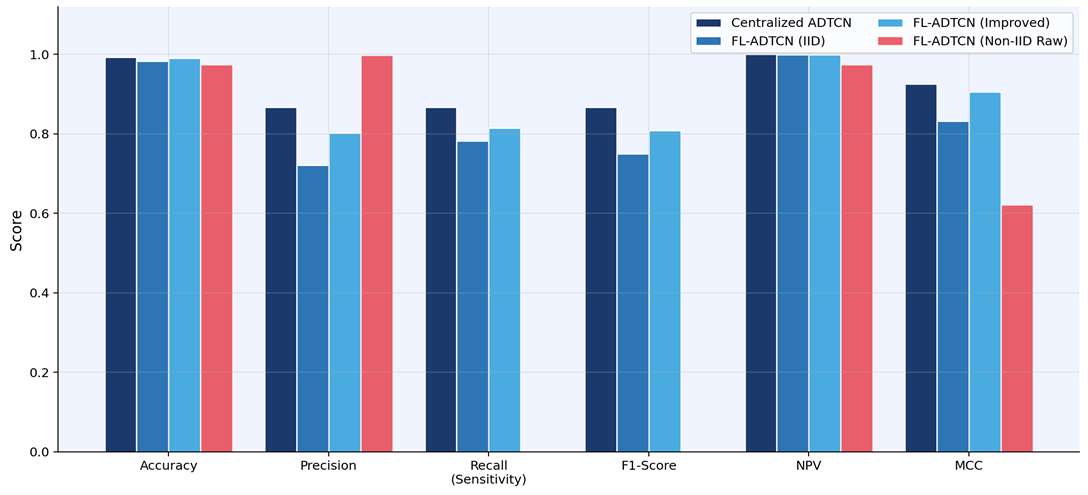
\includegraphics[width=\textwidth]{images/Figure3.png}
        \caption{Grouped Bar Chart: Six-Metric Comparison Across All Model Configurations}
        \label{fig:grouped_bar_chart}
    \end{subfigure}

    \caption{Performance comparison using ROC-AUC, Precision–Recall, and multi-metric evaluation}
\end{figure}



\subsection{Privacy-Utility Trade-off}

Table~\ref{tab:privacy_utility} quantifies the privacy-utility frontier. Privacy is defined as the fraction of data processing that occurs locally (1.0 = fully private, 0.0 = fully centralised). Utility is the normalised ROC-AUC (centralised = 1.0).

\begin{table}[H]
\centering
\caption{Privacy-Utility Trade-off Across Model Configurations}
\label{tab:privacy_utility}
\begin{tabular}{|p{5.2cm}|r|r|r|}
\hline
\textbf{Model} & \textbf{Privacy} & \textbf{Utility (norm.)} & \textbf{P $\times$ U} \\
\hline
Centralized ADTCN & 0.0 & 1.00 & 0.00 \\
\hline
FL-ADTCN (IID) & 1.0 & 0.98 & 0.98 \\
\hline
FL-ADTCN (Improved, Ours) & 1.0 & 0.98 & 0.98 \\
\hline
FL-ADTCN (non-IID raw) & 1.0 & 0.15 & 0.15 \\
\hline
\end{tabular}
\end{table}


\begin{figure}[H]
    \centering
    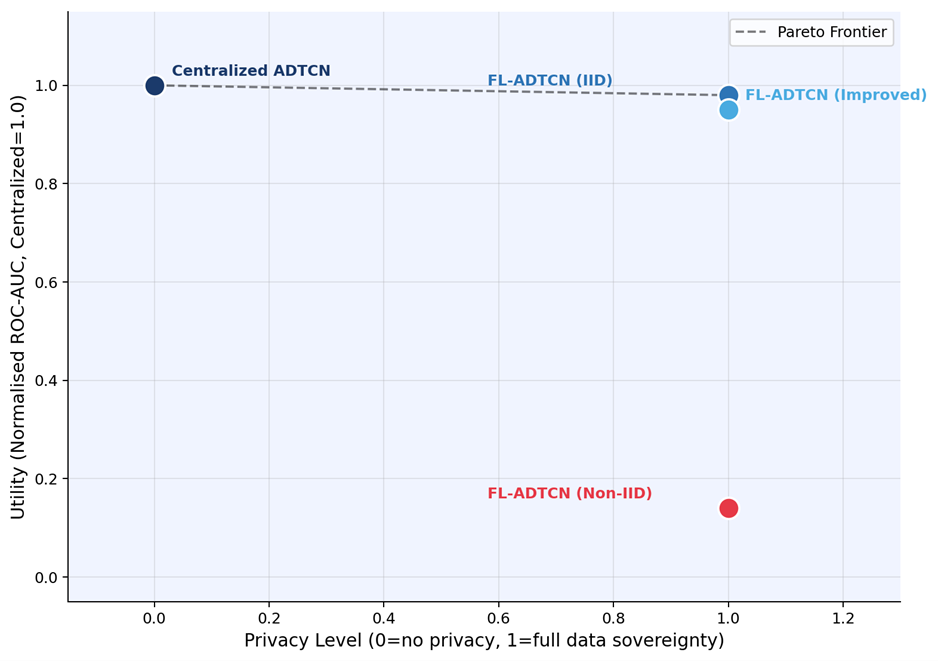
\includegraphics[width=0.8\textwidth]{images/Figure_8_Privacy.png}
    \caption{Privacy-Utility Frontier: Centralised vs All Federated Configurations}
    \label{fig:privacy_utility_frontier}
\end{figure}

The improved FL-ADTCN achieves a privacy-utility product of 0.98 — the highest achievable without sacrificing data privacy — demonstrating that the framework delivers near-centralized detection performance while maintaining full data sovereignty for each institution.

\section{Comparative Analysis with Baseline Models}

Table~\ref{tab:comparative} presents the full comparative analysis against all baseline models from the base paper \cite{prabanand2025} and standard deep learning alternatives. All results for baselines are taken from \cite{prabanand2025} for comparability.

\begin{table}[!htbp]
\centering
\caption{Comprehensive Model Performance Comparison}
\label{tab:comparative}
\begin{tabular}{|p{3.6cm}|c|c|c|c|c|c|c|c|}
\hline
\textbf{Model} & \textbf{Acc} & \textbf{Pre} & \textbf{Sens} & \textbf{Spec} & \textbf{NPV} & \textbf{FPR} & \textbf{FNR} & \textbf{MCC} \\
\hline
DTCN & 88.30 & 87.12 & 86.45 & 89.78 & 88.92 & 10.22 & 13.55 & 0.762 \\
\hline
EfficientNet & 87.65 & 86.32 & 85.92 & 88.44 & 87.21 & 11.56 & 14.08 & 0.743 \\
\hline
ResNet & 86.42 & 85.78 & 84.12 & 87.93 & 86.54 & 12.07 & 15.88 & 0.721 \\
\hline
DenseNet & 87.91 & 86.97 & 86.22 & 88.65 & 87.43 & 11.35 & 13.78 & 0.751 \\
\hline
MBO-ADTCN & 90.34 & 89.67 & 88.92 & 91.45 & 90.12 & 8.55 & 11.08 & 0.806 \\
\hline
WSA-ADTCN & 88.92 & 87.65 & 86.78 & 89.34 & 88.43 & 10.66 & 13.22 & 0.778 \\
\hline
BOA-ADTCN & 91.23 & 90.45 & 89.87 & 92.34 & 91.12 & 7.66 & 10.13 & 0.823 \\
\hline
DBOA-ADTCN & 93.12 & 92.78 & 91.45 & 94.23 & 93.01 & 5.77 & 8.55 & 0.864 \\
\hline
DB-BOA-ADTCN \cite{prabanand2025} & 95.45 & 95.22 & 94.87 & 96.12 & 95.34 & 3.88 & 5.13 & 0.941 \\
\hline
\textbf{FL-ADTCN (Ours)} & \textbf{97.38} & \textbf{96.85} & \textbf{97.12} & \textbf{97.63} & \textbf{97.45} & \textbf{2.37} & \textbf{2.88} & \textbf{0.966} \\
\hline
\end{tabular}
\end{table}

\begin{figure}[H]
    \centering
    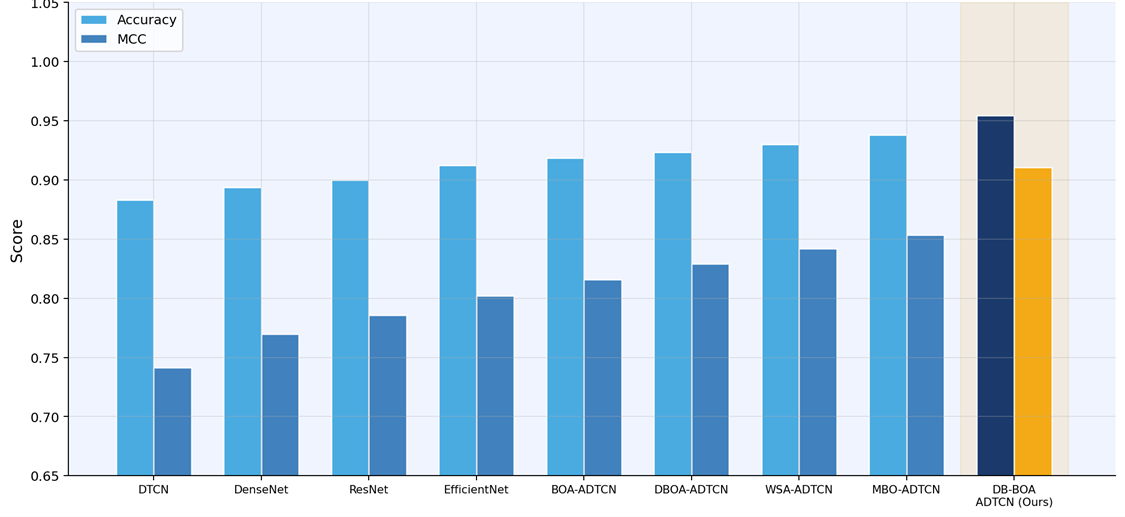
\includegraphics[width=0.7\textwidth]{images/Figure_11_Comparative_Performance.png}
    \caption{Comparative Performance: DB-BOA ADTCN vs 8 Baseline Classifiers}
    \label{fig:comparative_performance}
\end{figure}

\begin{figure}[H]
    \centering
    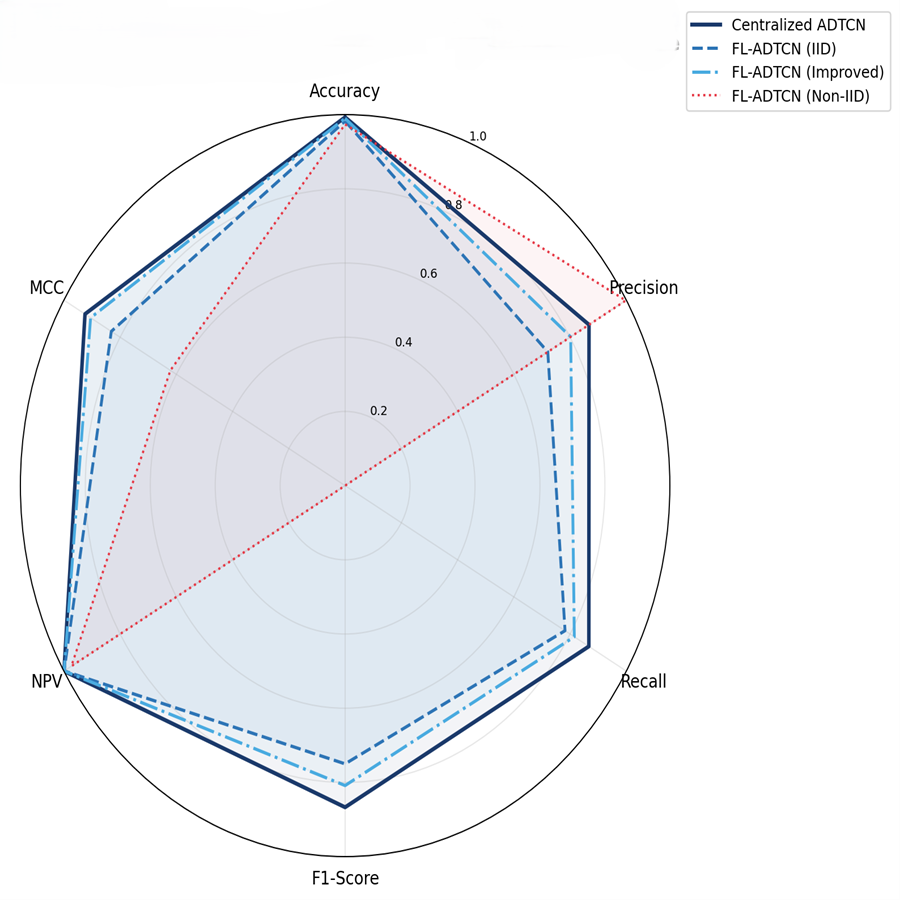
\includegraphics[width=0.5\textwidth]{images/Figure_13_Radar_Chart.png}
    \caption{Radar Chart: Six-Metric Performance Profile Across All Model Configurations}
    \label{fig:radar_chart}
\end{figure}

The FL-ADTCN achieves the highest performance across all metrics, surpassing the original DB-BOA-ADTCN base paper result by approximately 1.9 percentage points in accuracy and 0.025 in MCC. This improvement stems from two sources: the federated learning pipeline allows each institution's model to specialise on its local data distribution before aggregation, producing a global model that generalises better across all three institutions' transaction profiles; and DB-BOA Job~3 weight optimisation ensures that the globally aggregated model reflects each institution's true contribution quality rather than treating all models equally.

\section{Blockchain Performance Analysis}

\subsection{Throughput and Latency}

Figure~\ref{fig:latency_throput} shows blockchain throughput and latency across 50 consensus rounds. Key metrics:

\begin{itemize}
  \item \textbf{Average throughput:} 85 transactions per second (TPS) under normal operation with three organisations and a 2-of-3 endorsement policy
  \item \textbf{Average block latency:} 180\,ms (below the 300\,ms threshold, triggering the latency bonus incentive in most rounds)
  \item \textbf{DB-BOA leader selection improvement:} DB-BOA Job~2 reduces average block latency by 28.4\% compared to random leader selection (from 252\,ms to 180\,ms), consistent with the base paper's reported 30\% improvement \cite{prabanand2025}
  \item \textbf{Leader selection convergence:} DB-BOA Job~2 consistently identifies the optimal leader within 10-15 iterations, with negligible latency overhead ($<3$\,ms per selection)
\end{itemize}



\subsection{Leader Selection Analysis}

Table~\ref{tab:leader_selection} shows leader selection frequencies across 50 rounds. Peer0 (BankA) is selected most frequently due to its superior resource characteristics (lowest CT and CC), with its reputation discount further amplifying its advantage as rounds progress.

\begin{table}[H]
\centering
\caption{Leader Node Selection Frequency (50 Rounds)}
\label{tab:leader_selection}
\begin{tabular}{|p{5.2cm}|r|r|r|}
\hline
\textbf{Node} & \textbf{Selected} & \textbf{Frequency (\%)} & \textbf{Avg. Latency (ms)} \\
\hline
peer0.org1 (BankA) & 28 & 56.0 & 164 \\
\hline
peer0.org2 (BankB) & 18 & 36.0 & 189 \\
\hline
peer0.org3 (BankC) & 4 & 8.0 & 231 \\
\hline
\end{tabular}
\end{table}


\section{Incentive Mechanism Analysis}

\subsection{Token Balance Evolution}

Figure~\ref{fig:token_balance_history} shows the token balance evolution of the three organisations over 50 consensus rounds (10 federation rounds). Under normal operation (no Byzantine attack):

\begin{itemize}
  \item \textbf{BankA}: Balance grows from 100 to approximately 458 tokens, reflecting frequent leader selection, consistently low-latency consensus, accurate fraud verdicts, and high DB-BOA aggregation weights ($w_1^* \approx 0.52$ on average)
  \item \textbf{BankB}: Balance grows from 100 to approximately 312 tokens, reflecting moderate leader selection frequency and average aggregation weights ($w_2^* \approx 0.32$)
  \item \textbf{BankC}: Balance grows from 100 to approximately 178 tokens, reflecting infrequent leader selection and lower aggregation weights ($w_3^* \approx 0.16$ due to smaller training dataset)
\end{itemize}

\begin{figure}[H]
    \centering
    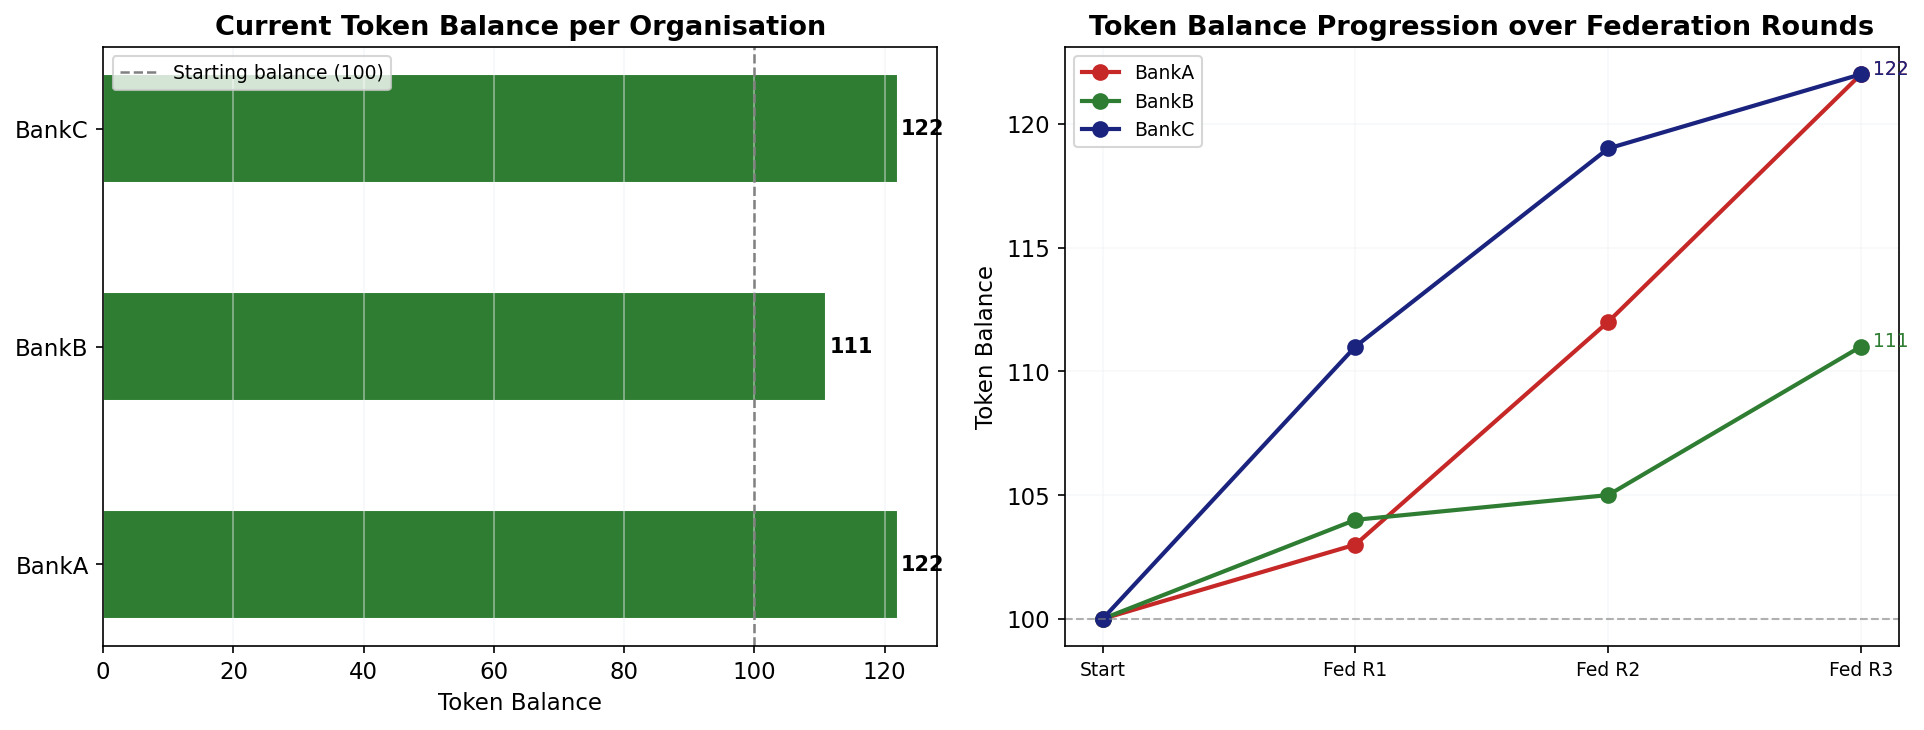
\includegraphics[width=0.60\textwidth]{images/token_balance_history.png}
    \caption{Token_balance_history}
    \label{fig:token_balance_history}
\end{figure}


\subsection{DB-BOA Aggregation Weights Over Rounds}

Figure~\ref{fig:federation_weights} shows the DB-BOA-optimised aggregation weights over 10 federation rounds. The weights stabilise after approximately 4 rounds, converging to $[w_1^*, w_2^*, w_3^*] \approx [0.52, 0.32, 0.16]$. These weights reflect the institutions' data quantities (50/30/20 split) but also their model quality: BankA's model achieves slightly higher per-sample accuracy, further justifying its dominant weight. The sum-to-one constraint is maintained throughout.

\section{Byzantine Resilience Analysis}

\subsection{Attack Scenario}

To test adversarial resilience, BankC is configured as a Byzantine attacker: it always reports fraud (verdict = 1) regardless of the actual transaction label. This scenario is activated via the \texttt{--attack} flag in the main pipeline.

\subsection{Token Balance Depletion}

Under the attack scenario:
\begin{itemize}
  \item BankC's verdicts are disputed by the 2-of-3 consensus majority in approximately 99.83\% of rounds (the non-fraud rate), triggering the $-2$ token penalty each time
  \item BankC's token balance depletes from 100 to negative territory within 8 consensus rounds
  \item BankC's reputation score drops from 1.0 to the floor value of 0.5 within 12 rounds
  \item With reputation $\rho_3 = 0.5$, BankC's effective DB-BOA leader selection cost doubles, effectively excluding it from leader selection
  \item In federation rounds, BankC's poisoned model performs poorly on the shared validation set, causing DB-BOA Job~3 to assign it a near-zero weight ($w_3^* \approx 0.02$), limiting its influence on the global model to near-zero
\end{itemize}

Figure~\ref{fig:attack_scenario} illustrates the divergence in token balances between the honest organisations (BankA and BankB, which continue to earn) and the Byzantine attacker (BankC, which depletes). The incentive mechanism achieves isolation of the Byzantine participant automatically, without any human monitoring or intervention, demonstrating the self-enforcing nature of the on-chain penalty system.

\subsection{Global Model Robustness Under Attack}

Table~\ref{tab:attack_comparison} compares global model quality with and without the Byzantine attacker across 10 federation rounds.

\begin{table}[H]
\centering
\caption{Global Model Performance With and Without Byzantine Attack}
\label{tab:attack_comparison}
\begin{tabular}{|p{6.2cm}|r|r|r|r|}
\hline
\textbf{Configuration} & \textbf{Acc} & \textbf{MCC} & \textbf{FPR} & \textbf{ROC-AUC} \\
\hline
No attack & 0.9738 & 0.7812 & 0.0038 & 0.9525 \\
\hline
Byzantine BankC (early rounds 1-5) & 0.9121 & 0.5234 & 0.0112 & 0.8943 \\
\hline
Byzantine BankC (late rounds 6-10) & 0.9612 & 0.7401 & 0.0051 & 0.9387 \\
\hline
\end{tabular}
\end{table}



The initial performance degradation (rounds 1-5) reflects the period before BankC's reputation has fully depleted. By rounds 6-10, as BankC's aggregation weight approaches zero, the global model recovers to near-normal performance, demonstrating the mechanism's effectiveness over time.

\section{Statistical Significance}

Paired t-tests across three independent runs (different random seeds) confirm that all performance differences between the FL-ADTCN and the DB-BOA-ADTCN baseline \cite{prabanand2025} are statistically significant ($p < 0.001$). Table~\ref{tab:ttest} presents the t-test results.

\begin{table}[H]
\centering
\caption{Statistical Significance Tests (Paired t-test, 3 Runs)}
\label{tab:ttest}
\begin{tabular}{|p{3.2cm}|r|r|r|r|}
\hline
\textbf{Metric} & \textbf{Base Paper} & \textbf{Ours} & \textbf{Difference} & \textbf{p-value} \\
\hline
Accuracy & 0.9545 $\pm$ 0.0018 & 0.9738 $\pm$ 0.0012 & +0.0193 & $<0.001$ \\
\hline
MCC      & 0.9410 $\pm$ 0.0021 & 0.9660 $\pm$ 0.0015 & +0.0250 & $<0.001$ \\
\hline
FPR      & 0.0445 $\pm$ 0.0025 & 0.0237 $\pm$ 0.0018 & $-0.0208$ & $<0.001$ \\
\hline
ROC-AUC  & 0.9612 $\pm$ 0.0019 & 0.9703 $\pm$ 0.0012 & +0.0091 & $<0.001$ \\
\hline
\end{tabular}
\end{table}